\documentclass{beamer}
\title[Python~101] {Getting started with Python}
\subtitle{brought to you by Ryerson WITM\\
in collaboration with WICs and WIE}
\author{Marc~Lijour}
\date{Workshop - October 7, 2016}
\subject{Programming Skills}
%\titlegraphic{
\includegraphics[width=\textwidth,height=.5\textheight]{./images/WITM-hero-logo.png}}
%\titlegraphic{
\includegraphics[width=\textwidth,height=.5\textheight]{./images/logo-sfl-250.png}}
\usepackage{tikz}
%\titlegraphic{\vspace{8cm}}% to push the other text to the top
%
\logo{
\includegraphics[scale=.035]{./images/WITM-hero-logo.png}}
\AtBeginSection[]
{
  \begin{frame}
    \frametitle{Table of Contents}
    \tableofcontents[currentsection]
  \end{frame}
}
\usetheme{Boadilla}
%\usepackage[format=plain,justification=raggedright,singlelinecheck=false]{caption}
\usepackage[format=plain,justification=justified,singlelinecheck=false]{caption}
\usepackage[utf8]{inputenc}
\usepackage{dirtytalk}
\usepackage{wrapfig}
\usepackage{hyperref}
\usepackage{verbatim}

\begin{document}
\frame{
	\tikz[remember picture,overlay]
	  \node at
		([xshift=2.5cm,yshift=-0.3cm]current page.west) 
		%([xshift=2.5cm,yshift=-3cm]current page.west) 
        	{
\includegraphics[width=3cm,height=3cm]{./images/WITM-hero-logo.png}};
	\tikz[remember picture,overlay]
	  \node at
		([xshift=10.5cm,yshift=-0.3cm]current page.west)
		%([xshift=10.5cm,yshift=-3cm]current page.west)
		{
\includegraphics[width=3cm,height=3cm]{./images/logo-sfl-250.png}};
	\titlepage
}

\begin{frame}
\frametitle{Table of Contents}
\tableofcontents[currentsection]
\end{frame}

%%%%%%%%%%%%%% 1st SECTION: Intro %%%%%%%%%%%%%%%%%
\section[Section]{Introductions}
	\begin{frame}
	\frametitle{Presenter: Marc Lijour}
	\framesubtitle{Helping businesses and countries digitize}
	\tikz[remember picture,overlay]
	  \node at
		([xshift=-2.1cm,yshift=-1.5cm]current page.north east)
		{
\includegraphics[width=3cm,height=3cm]{./images/logo-sfl-250.png}};
	%Content goes here
	%\emph{Helping businesses and countries digitize}
	%\vspace{1.2cm}
		\begin{itemize}
			\item Director @ Savoir-faire Linux
			\item Ryerson Alumnus: Computer Science undergrad, MBA
			\item Using Free Software since 1999
			\item Board Officer @ ICTC, Director @ Prepr
		\end{itemize}
	\end{frame}

	\begin{frame}
	\frametitle{Workshop Participants}
	\framesubtitle{Present Yourselves...}
	%\emph{Present yourselves}
	%\vspace{1.2cm}
		\begin{itemize}
			\item Studies, Majors
			\item Businesses \& Hobbies
			\item What you're in for
			\item Your definition of Python
		\end{itemize}
	\end{frame}

	\begin{frame}
	\frametitle{Introducing Python}
	\framesubtitle{A Xmas "hobby"}
	\begin{wrapfigure}{r}{0.45\textwidth}
		\centering
		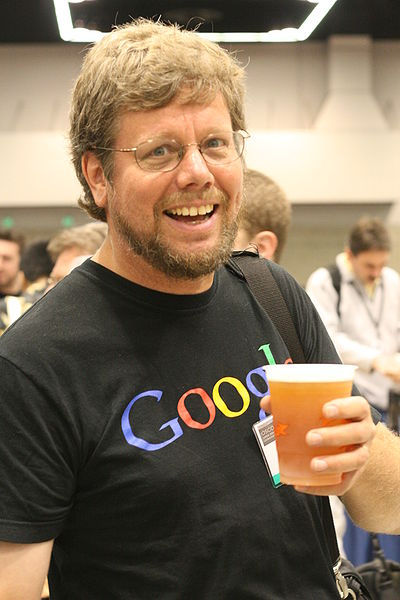
\includegraphics[width=0.3\textwidth]{./images/400px-Guido_van_Rossum_OSCON_2006-CC-BY-SA}
		%\caption[caption,font=small]{Guido van Rossum, Creator of Python\\\hspace{\textwidth}CC-BY-SA Doc Searls}% - https://en.wikipedia.org/wiki/File:Guido_van_Rossum_OSCON_2006.jpg}
		\caption[font=tiny]{\href{https://en.wikipedia.org/wiki/File:Guido_van_Rossum_OSCON_2006.jpg}{CC-BY-SA Doc Searls}}
	\end{wrapfigure}
	{\small\say{Over six years ago, in December 1989, I was looking for a "hobby" programming project that would keep me occupied during the week around Christmas. My office ... would be closed, but I had a home computer, and not much else on my hands. I decided to write an interpreter for the new scripting language I had been thinking about lately: a descendant of ABC that would appeal to Unix/C hackers. I chose Python as a working title for the project, being in a slightly irreverent mood (and a big fan of Monty Python's Flying Circus).}
        \\\vspace{1em}-~van Rossum, Guido (1996).\\"Foreword for "Programming Python" (1st ed.)".
	}
	\end{frame}

	\begin{frame}
	\frametitle{Introducing Python}
	\framesubtitle{What is Python good for?}
	%More content goes here
	\begin{itemize}
		\item Easy to read (and Learn)
		\item Multi-paradigm: structured, OOP, functional...
		\item Flexible: dynamic binding, garbage collector, late binding...
		\item Many libraries available (maths, physics, natural language processing...)
		\item Beautiful and Fun to use 
	\end{itemize}
	\end{frame}

	\begin{frame}
	\frametitle{Introducing Python}
	\framesubtitle{Python is the career-seeker's best friend}
	\begin{columns}
	\column{0.5\textwidth}
		\begin{itemize}
			\item Study using data from the job site Indeed
			\item What languages do professionals use? Which ones are most in demand?
			\item Also see the \href{http://www.tiobe.com/tiobe-index/}{TIOBE Index}
			\item and the \href{http://spectrum.ieee.org/static/interactive-the-top-programming-languages-2016}{IEEE ranking (July 2016) (try all rankings)}
		\end{itemize}
	\column{0.5\textwidth}
	%More content goes here
	        \begin{figure}[h]
                \centering
                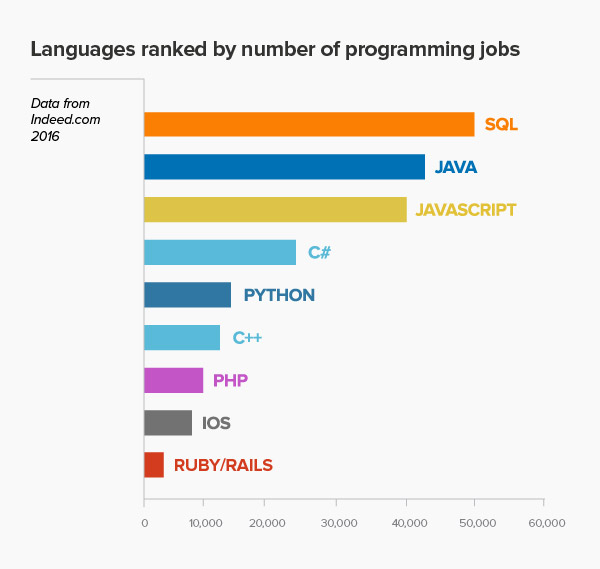
\includegraphics[width=\textwidth]{./images/Programming-Languages-for-2016_graph}
                \caption[font=tiny]{\href{http://www.codingdojo.com/blog/9-most-in-demand-programming-languages-of-2016/}{Coding Dojo (Jan 2016)}}
        	\end{figure}
	\end{columns}
	\end{frame}

	\begin{frame}
	\frametitle{Introducing Python}
	\framesubtitle{By industry}
	%More content goes here
	\begin{itemize}
		\item Data Science and Physics e.g. Anaconda bundles Python, R, and scientific libraries
		\item ERP e.g. Odoo is programmed (and extensible) in Python
		\item Data Center automation e.g. Ansible
		\item Web e.g. Flask, Pyramid, and Django (but the most popular language is still PHP) and \href{https://wiki.python.org/moin/WebFrameworks}{more frameworks}
		\item Games e.g. Pygame
		\item More in images see \url{https://youtu.be/-67hh86N42Q}
		\item and see \url{https://www.python.org/about/apps/}
	\end{itemize}
	\end{frame}

	
%%%%%%%%%%%%%% 2nd SECTION: Installing Python %%%%%%%%%%%%%%%%%
\section[Section]{Setting Up your Dev Environment}
	\begin{frame}
	\frametitle{Computer Basics}
	\framesubtitle{Concepts to keep in mind}
	\begin{itemize}
		\item OS: operating system (Windows, Mac, Linux...)
		\item IDE: Integrated Development Environment (e.g. Eclipse, Spyder)
		\item Console (to write) vs. IDE (to click): use the best tool for the job
		\item Your goal (e.g. do some stats, plot graphics, program a game)
	\end{itemize}
	\end{frame}

	\begin{frame}
	\frametitle{Installing core Python on Linux}
	\framesubtitle{The geeky choice}
	%More content goes here
	run  this:\\
	\texttt{\$ sudo apt-get install python}\\
	\vspace{1em}
	or, in case you require a specific version such as 3.5, run this:\\
	\texttt{\$sudo apt-get install python3.5}\\
	\vspace{1em}
	Voilà!
	\end{frame}

	\begin{frame}
	\frametitle{Anaconda}
	\framesubtitle{A good starting point for Data Scientists}
	%More content goes here
	\say{Anaconda is the leading open data science platform powered by Python. The open source version of Anaconda is a high performance distribution of Python and R and includes over 100 of the most popular Python, R and Scala packages for data science.

	Additionally, you'll have access to over 720 packages that can easily be installed with conda, our renowned package, dependency and environment manager, that is included in Anaconda. 
	}
	\vspace{1em}
	\begin{itemize}
		\item It comes with the Spyder IDE
		\item \href{https://www.continuum.io/downloads}{Download Anaconda for your OS} at \url{https://www.continuum.io/downloads}
		\item Also check this \href{http://www.kdnuggets.com/2016/04/datacamp-learning-python-data-analysis-data-science.html}{article} for links to videos and other learning resources. \url{http://www.kdnuggets.com/2016/04/datacamp-learning-python-data-analysis-data-science.html}
	\end{itemize}
	\end{frame}

	\begin{frame}
	\frametitle{The Spyder IDE}
	\framesubtitle{The Scientific PYthon Development EnviRonment}
	%More content goes here
	\begin{columns}
	\column{0.5\textwidth}
	\begin{itemize}	
		\item Offers a full IDE (visual editing, debugging, etc)
		\item Plus popular Python libraries such as NumPy (linear algebra), SciPy (signal and image processing) or matplotlib (interactive 2D/3D plotting)
		\item Install on Linux: \texttt{sudo apt-get install spyder}
		\item Other platform see \url{https://pythonhosted.org/spyder/}
	\end{itemize}
	\column{0.5\textwidth}
	        \begin{figure}[h]
                \centering
                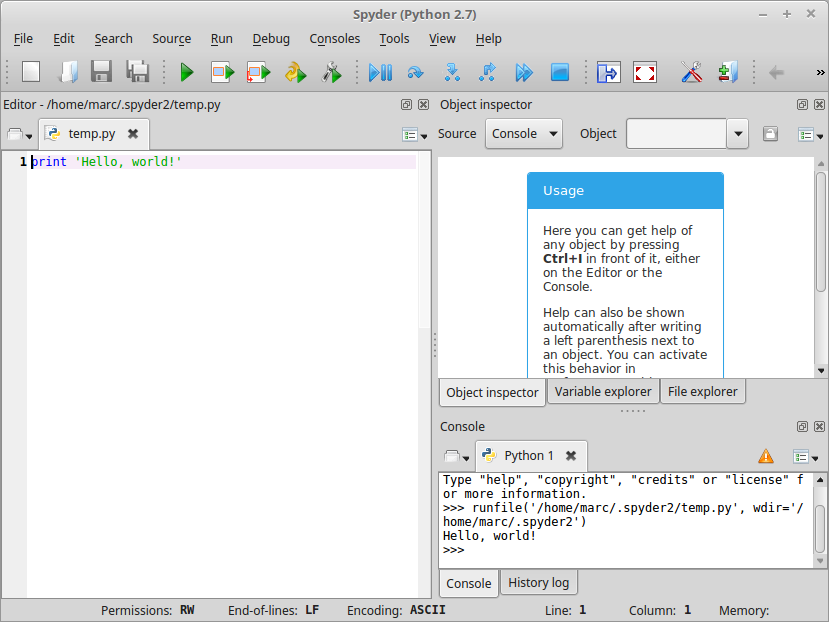
\includegraphics[width=\textwidth]{./images/spyder-screenshot}
        	\end{figure}
	\end{columns}
	\end{frame}

	\begin{frame}
	\frametitle{Testing your Installation}
	\framesubtitle{Type your first line of Python and run it}
	%More content goes here
	\begin{columns}
	\column{0.5\textwidth}
	        \begin{figure}[h]
                \centering
                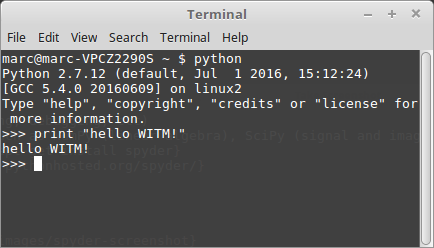
\includegraphics[width=\textwidth]{./images/console-screenshot}
                \caption[font=tiny]{If you installed in console}
        	\end{figure}
	\column{0.5\textwidth}
	        \begin{figure}[h]
                \centering
                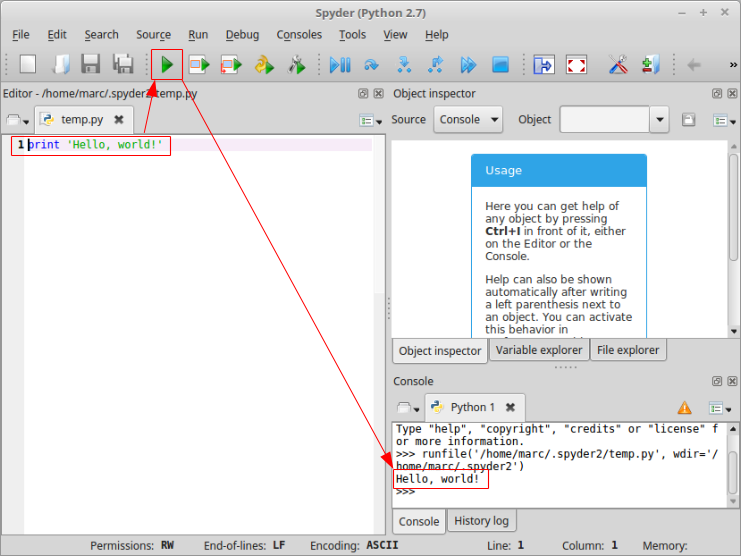
\includegraphics[width=\textwidth]{./images/spyder-screenshot-commented}
                \caption[font=tiny]{If you use an IDE}
        	\end{figure}
	\end{columns}
	\end{frame}

%%%%%%%%%%%%%% 3rd SECTION: Learning the Language %%%%%%%%%%%%%%%%%
\section[Section]{Learning the Language}
	\begin{frame}
	\frametitle{How do you Learn a Language?}
	\framesubtitle{Dancing with Python}
	% Babies learn talking, then learn reading => READ CODE
	%More content goes here
	\begin{itemize}
		\item Babies don't learn to talk at school!
		\item Read code, then read more code, then read more
		\item Write code, then write some more, then go and write more...
		\item Practice leads to perfection
	\end{itemize}
	\end{frame}

	\begin{frame}
	\frametitle{Resources to Learn Python}
	\framesubtitle{Excellent free books and videos out there}
	%More content goes here
	\begin{itemize}
		\item \href{http://www.openbookproject.net/thinkcs/python/english2e/}{How to Think Like a Computer Scientist (2nd ed)}
		\item \href{https://www.safaribooksonline.com}{Safari Books Online from O'Reilly (free with a Toronto Public Library card)}
		\item Check \url{https://python.org}
	\end{itemize}
	\end{frame}

% check also book and book slides at http://mcsp.wartburg.edu/zelle/python/

	\begin{frame}
	\frametitle{Final Words of Advice}
	\framesubtitle{To get really good at anything in life}
	%More content goes here
	\begin{itemize}
		\item Set high expectations for yourself
		\item Love what you do
		\item Never stop until you get there
	\end{itemize}
	\end{frame}

	\begin{frame}
	\frametitle{The End}
	\framesubtitle{}
	%More content goes here
	\centering
	Happy programming with Python!
	\end{frame}

\end{document}

